\documentclass[11pt,a4paper]{report}

% packages
\usepackage[left=20mm, right=15mm, top=10mm, bottom=15mm]{geometry}
\usepackage{tocloft}
\usepackage{graphicx}
\usepackage{subcaption}
\usepackage{amsmath}
\usepackage{setspace}
\usepackage{makecell}
\usepackage[utf8]{inputenc}
% \usepackage{algorithmic}
\usepackage[english]{babel}
\usepackage{amsthm}
\usepackage{arevmath}     % For math symbols
\usepackage[noend]{algpseudocode}
\usepackage{amssymb}
\usepackage{algorithm2e}


\theoremstyle{definition}
\newtheorem{definition}{Definition}[section]

\theoremstyle{remark}
\newtheorem*{remark}{Remark}

\begin{document}

    \tableofcontents

    
    \section{Introduction}
    The objective of this medium-sized scientific software engineering project is to implement the power function while approaching the problem from first principles. Tasks like \textbf{documenting}, \textbf{versioning}, and \textbf{testing} are considered first class citizens.
    
    System, Software system, Eternity all refer to the same time.
    
    \chapter{Power Function}
    
        \begin{definition}
            The \textbf{power function} is defined as the function that takes any numbers $x$ and $y$ as input, raises $x$ to $y$, and returns $x^y$ as output.
        \end{definition}
    
        The power function is a transcendental function and cannot be expressed in terms of a finite sequence of the algebraic operations of raising to a power, division, multiplication, addition, subtraction, and root extraction [wikipedia].
        
        All the exponentiation rules are applicable here.
        
        \section{Domain and Co-domain} [algoritms website]
        The domains and co-domains of $x$ and $y$ vary as follows:
        
        \begin{itemize}
            \item If \textbf{base $x$ is a positive real number}, then $y$ belongs to the set of all reals numbers.
            
            The corresponding range is the set of all positive real numbers.
            
            \item If \textbf{base $x$ is zero}, then $y$ belongs to the set of non-negative real numbers.
            
            This is because a negative $y$ would lead to division by zero.
            
            \item If \textbf{base $x$ is negative}, then $y$ may only have to certain values:

                    \begin{itemize}
                        \item $y$ \textbf{may be} any integer.
                        
                        \item $y$ \textbf{may be} a fraction of the form $a/b$ where \emph{b} is odd.
                        
                        \item $y$ \textbf{may not be} a fraction of the form $a/b$ where \emph{b} is even.
                        
                        \item $y$ \textbf{may not be} an irrational number. 
                        
                    \end{itemize}
            
        \end{itemize}
        
        !!!! Please add the boundary cases here.
        
        \section{Context of use Model}
            The context of use is a description of the condtions under which the software system will be used under the normal working circumstances. 
            A context of use model is a useful tool to explore and understand the details and boundaries of a project. 
            % ["https://www.edrawmax.com/context-diagram/#:~:text=What%20are%20the%20Benefits%20of%20a%20Context%20Diagram%3F,skills%20or%20knowledge%20to%20understand%20a%20context%20diagram.]
            
            There is currently no standard for representing the context of use. A context diagram is however a suitable candidate for mind mapping. 
            
            Fig 1. is a context diagram for this project built using the [gitmind tool]. It focusses on the users of the systems and the environments where this system will be operated. The users block is subdivided into blocks representing the potential users of the system and their requirements for effective and efficient completion of thei responsibilities.
            
            The environment block explores the different system environments needed to perform different tasks. In particular, the developers, testers and, maintainer require a Technical environment. The end-user however doesn't require anything more than the general environment.
        
            \begin{figure}[htbp]
                \centering
                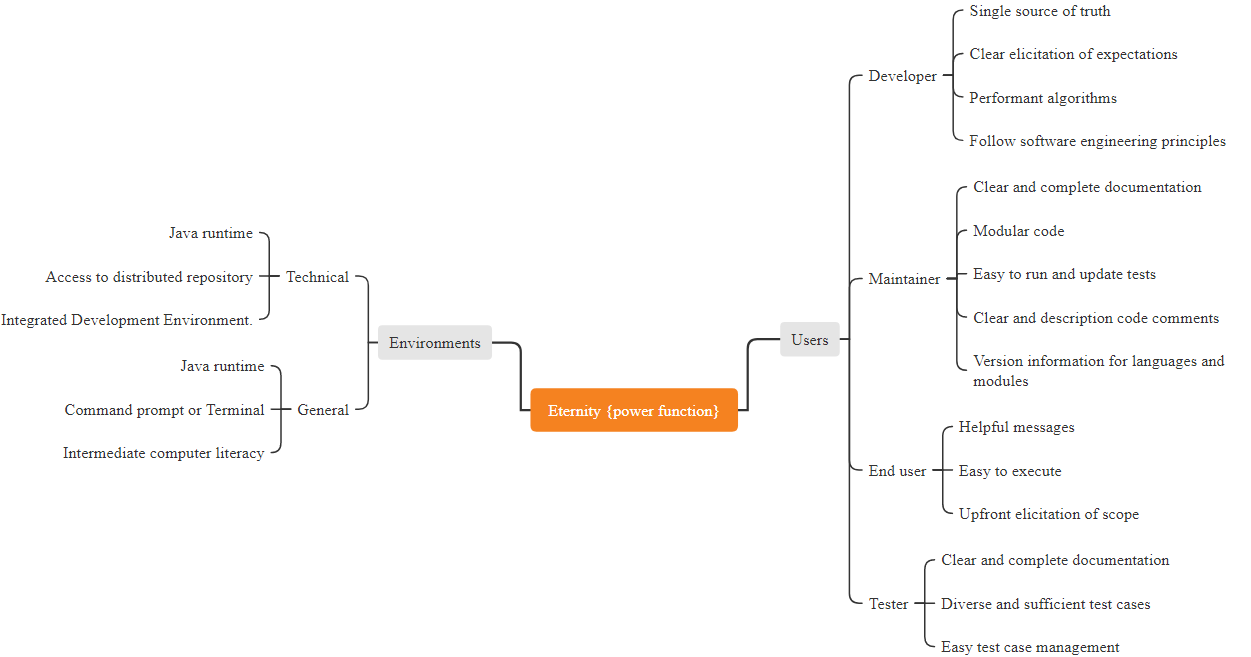
\includegraphics[width=\linewidth]{lecture-10/Context_of_use.PNG}
                \caption{Context of use for Eternity.}
                \label{fig:context_of_use}
            \end{figure}


\end{document}